\documentclass[a4paper,twoside,11pt]{article}
\usepackage{a4wide,graphicx,fancyhdr,amsmath,amssymb}

%----------------------- Macros and Definitions --------------------------

\setlength\headheight{20pt}
\addtolength\topmargin{-10pt}
\addtolength\footskip{20pt}

\newcommand{\N}{\mathbb{N}}
\newcommand{\ch}{\mathcal{CH}}

\newcommand{\solution}[1]{\noindent{\bf Solution to Exercise #1:}}

\fancypagestyle{plain}{%
\fancyhf{}
\fancyhead[LO,RE]{\sffamily\bfseries\large technische universiteit eindhoven}
\fancyhead[RO,LE]{\sffamily\bfseries\large 2IN35 VLSI}
\fancyfoot[LO,RE]{\sffamily\bfseries\large department of mathematics and computer science}
\fancyfoot[RO,LE]{\sffamily\bfseries\thepage}
\renewcommand{\headrulewidth}{0pt}
\renewcommand{\footrulewidth}{0pt}
}

\pagestyle{fancy}
\fancyhf{}
\fancyhead[RO,LE]{\sffamily\bfseries\large technische universiteit eindhoven}
\fancyhead[LO,RE]{\sffamily\bfseries\large 2IN35 VLSI}
\fancyfoot[LO,RE]{\sffamily\bfseries\large department of mathematics and computer science}
\fancyfoot[RO,LE]{\sffamily\bfseries\thepage}
\renewcommand{\headrulewidth}{1pt}
\renewcommand{\footrulewidth}{0pt}

\def\addsquare#1{\tikz\node[draw]{#1};} 

%-------------------------------- Title ----------------------------------

\title{\vspace{-\baselineskip}\sffamily\bfseries Assignment 3}
\author{
	Rick Veens \qquad Studentno: 0912292\\
	\texttt{r.veens@student.tue.nl}
	\and
	Barry de Bruin \qquad Studentno: -\\
	\texttt{-@student.tue.nl}
}

\date{\today}

\setlength\parindent{0pt}

%--------------------------------- Text ----------------------------------

\begin{document}
\maketitle
\newpage

\section*{Lab assignment 3a}
\subsection*{1. Requirements}
The assignment is to design and implement a FIR filter named filter that:
\begin{enumerate}
\item Uses as little resources as possible and is maximally sequential. In particular at most 1
multiplier may be used.
\item Conforms to the 4-phase asynchronous protocol for both input and output.
\item Can run at a clock frequency of 100 Mhz.
\item Honors changes in the coefficients (after a finite delay).
\item May produce a finite length interval of start-up noise
\end{enumerate}

\subsubsection*{1.1 Analysis of requirements}
The FIR filter should make use of only one DSP-unit, since the internal clock frequency is significantly higher than the expected sample rate. Furthermore the coefficients should not be buffered but must be connected as wires instead of buffering them in registers. This ensures that requirement 1 and 4 can be satisfied. For requirement 3, the clock frequency should be at least 100MHz, which will be checked in the post-synthesis report. Lastly, the asynchronous ack/req protocol will be used since there needs to be some synchronization between the testbench (44.1KHz sample rate) and the filter (100MHz sample rate).


\subsection*{2. System architecture}
Figure one shows the global architecture of the FIR filter. 
\begin{figure}[h]
	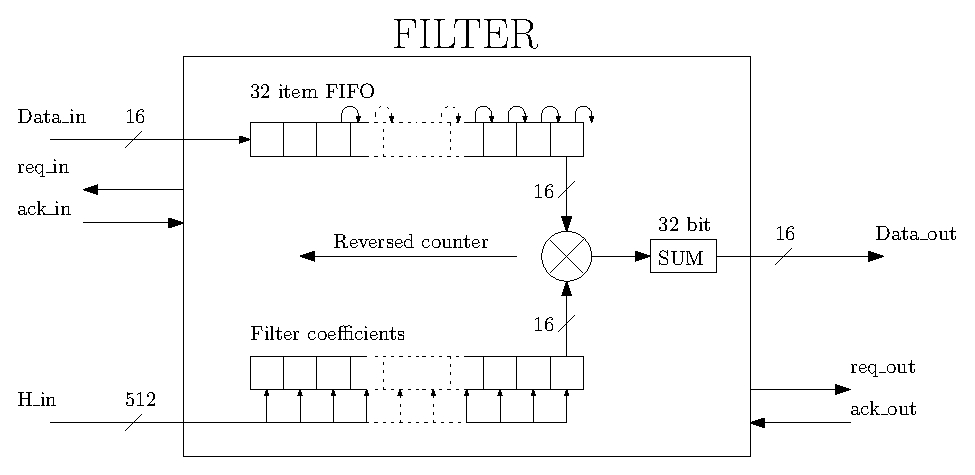
\includegraphics[scale = 1]{Images/3a_blockdiagram}
    \caption{System overview}
\end{figure}

Unlike the FIR filter of lab2, the filter has only one tap. After each clock edge the multiplier/accumulator will multiply a sample that is stored in the memory with it's corresponding filter coefficient. An index makes sure that this operation moves through the FIFO in 32 clock cycles. The index sample is also shifted one place to the right. After 32 cycles the last tap has  been calculated and the first place in the FIFO is empty. The system will output the calculated sample, and request a new data item, which will be put on the first index.\\ 

The whole procedure will then restart.
\subsection*{4. Design choices}

\subsection*{5. Functional correctness}
all requirements?

\subsection*{6. Resource usage}


\subsection*{7. System throughput and latency}
 (min) sample time Ts and (max) sample
frequency fs, both after synthesis and after placement \& routing.

\subsection*{8. Simulation results}
Time en FFT plot


\newpage
\section*{Lab assignment 3b}
\subsection*{1. Requirements}
The specific requirements for the strength reduced FIR filter are:
\begin{enumerate}
\item The design may use at most 3 multipliers.
\item Conforms to the 4-phase asynchronous handshake protocol for both input and output.
\item Can run at a clock frequency of 100 Mhz.
\item Should have about 4 times the sample frequency as the sequential implementation.
\item Honors changes in the coefficients (after a finite delay).
\item May produce a finite length interval of start-up noise.
\end{enumerate}


\newpage
\section*{Comparison between two filters}
In your final report, compare the output signals of the strength reduced filter with the output of the sequential filter, by generating a difference signal for a representative subset of
samples. Make sure you align the outputs correctly, because the amount of start-up noise of
the 2 implementations may differ. If the difference signal is non-zero, explain the differences.
Further reporting guidelines are on the course’s website.

\newpage
\section*{Appendix}
all verilog code



\end{document}
